\documentclass[red]{beamer}

\usepackage[italian]{babel}
\usepackage[utf8]{inputenc}
\usepackage{pgf}

\graphicspath{{./images/}}

\newtheorem{defs}{Definizione}[section]

\mode<presentation>{
    \usetheme[left]{Marburg}
    \useinnertheme[shadow]{rounded}
}

\AtBeginSubsection[]
{
  \begin{frame}<beamer>{Contenuti}
    \tableofcontents[currentsection,currentsubsection]
  \end{frame}
}

\title[Software per segnali radioastronomici]{Sviluppo di un software per l'analisi real-time di dati
radioastronomici su macchine multicore}
\author{Stéphane Bisinger}


\begin{document}

\begin{frame}
	\titlepage
\end{frame}

\begin{frame}{Riassunto}
	\tableofcontents
\end{frame}

\section{Teoria}
\subsection{Analisi dei segnali}
\begin{frame}{Cosa sono i segnali?}
	\transdissolve<3>
	\begin{defs} \label{def:signal}
		Si dice segnale una qualunque quantità che varia nel tempo o nello spazio.
	\end{defs}
	\pause

	Ad esempio un suono è un segnale frutto della variazione di pressione dell'aria nel tempo.
	\pause
	\begin{center}
		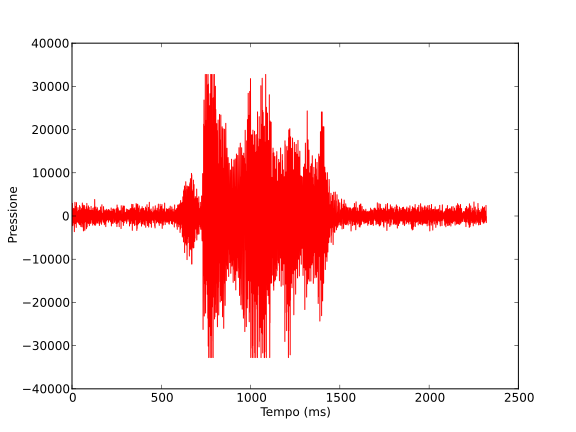
\includegraphics[width=0.7\textwidth]{img/segnale}
	\end{center}
\end{frame}

\begin{frame}{Come si analizza un segnale?}
	\transdissolve<4>
	\begin{itemize}
		\item Un qualunque segnale pu\`o essere espresso come somma pesata di
			sinusoidi. \pause
		\item Quindi un segnale pu\`o essere espresso in relazione alla frequenza
			delle sinusoidi parte del segnale \pause $->$ Rappresentazione del segnale nel
			dominio delle frequenze. \pause
	\end{itemize}
	\begin{center}
		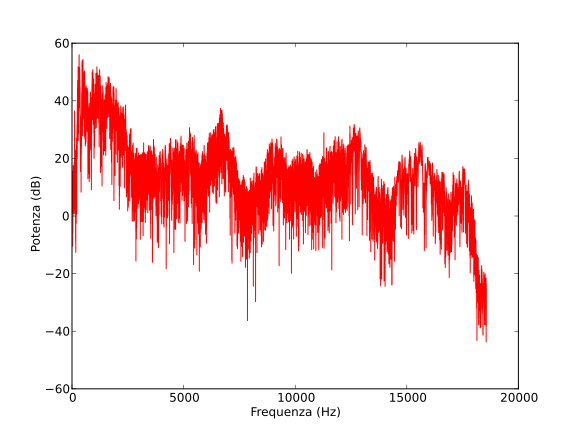
\includegraphics[width=0.7\textwidth]{img/frequenza}
	\end{center}
\end{frame}

\subsection{Radioastronomia}
\begin{frame}{I radiotelescopi}
	Un radiotelescopio osserva le onde elettromagnetiche provenienti dallo spazio
	con frequenze comprese tra i 70 Mhz ed i 43 Ghz, dette onde
	\emph{radio}.
	\begin{center}
		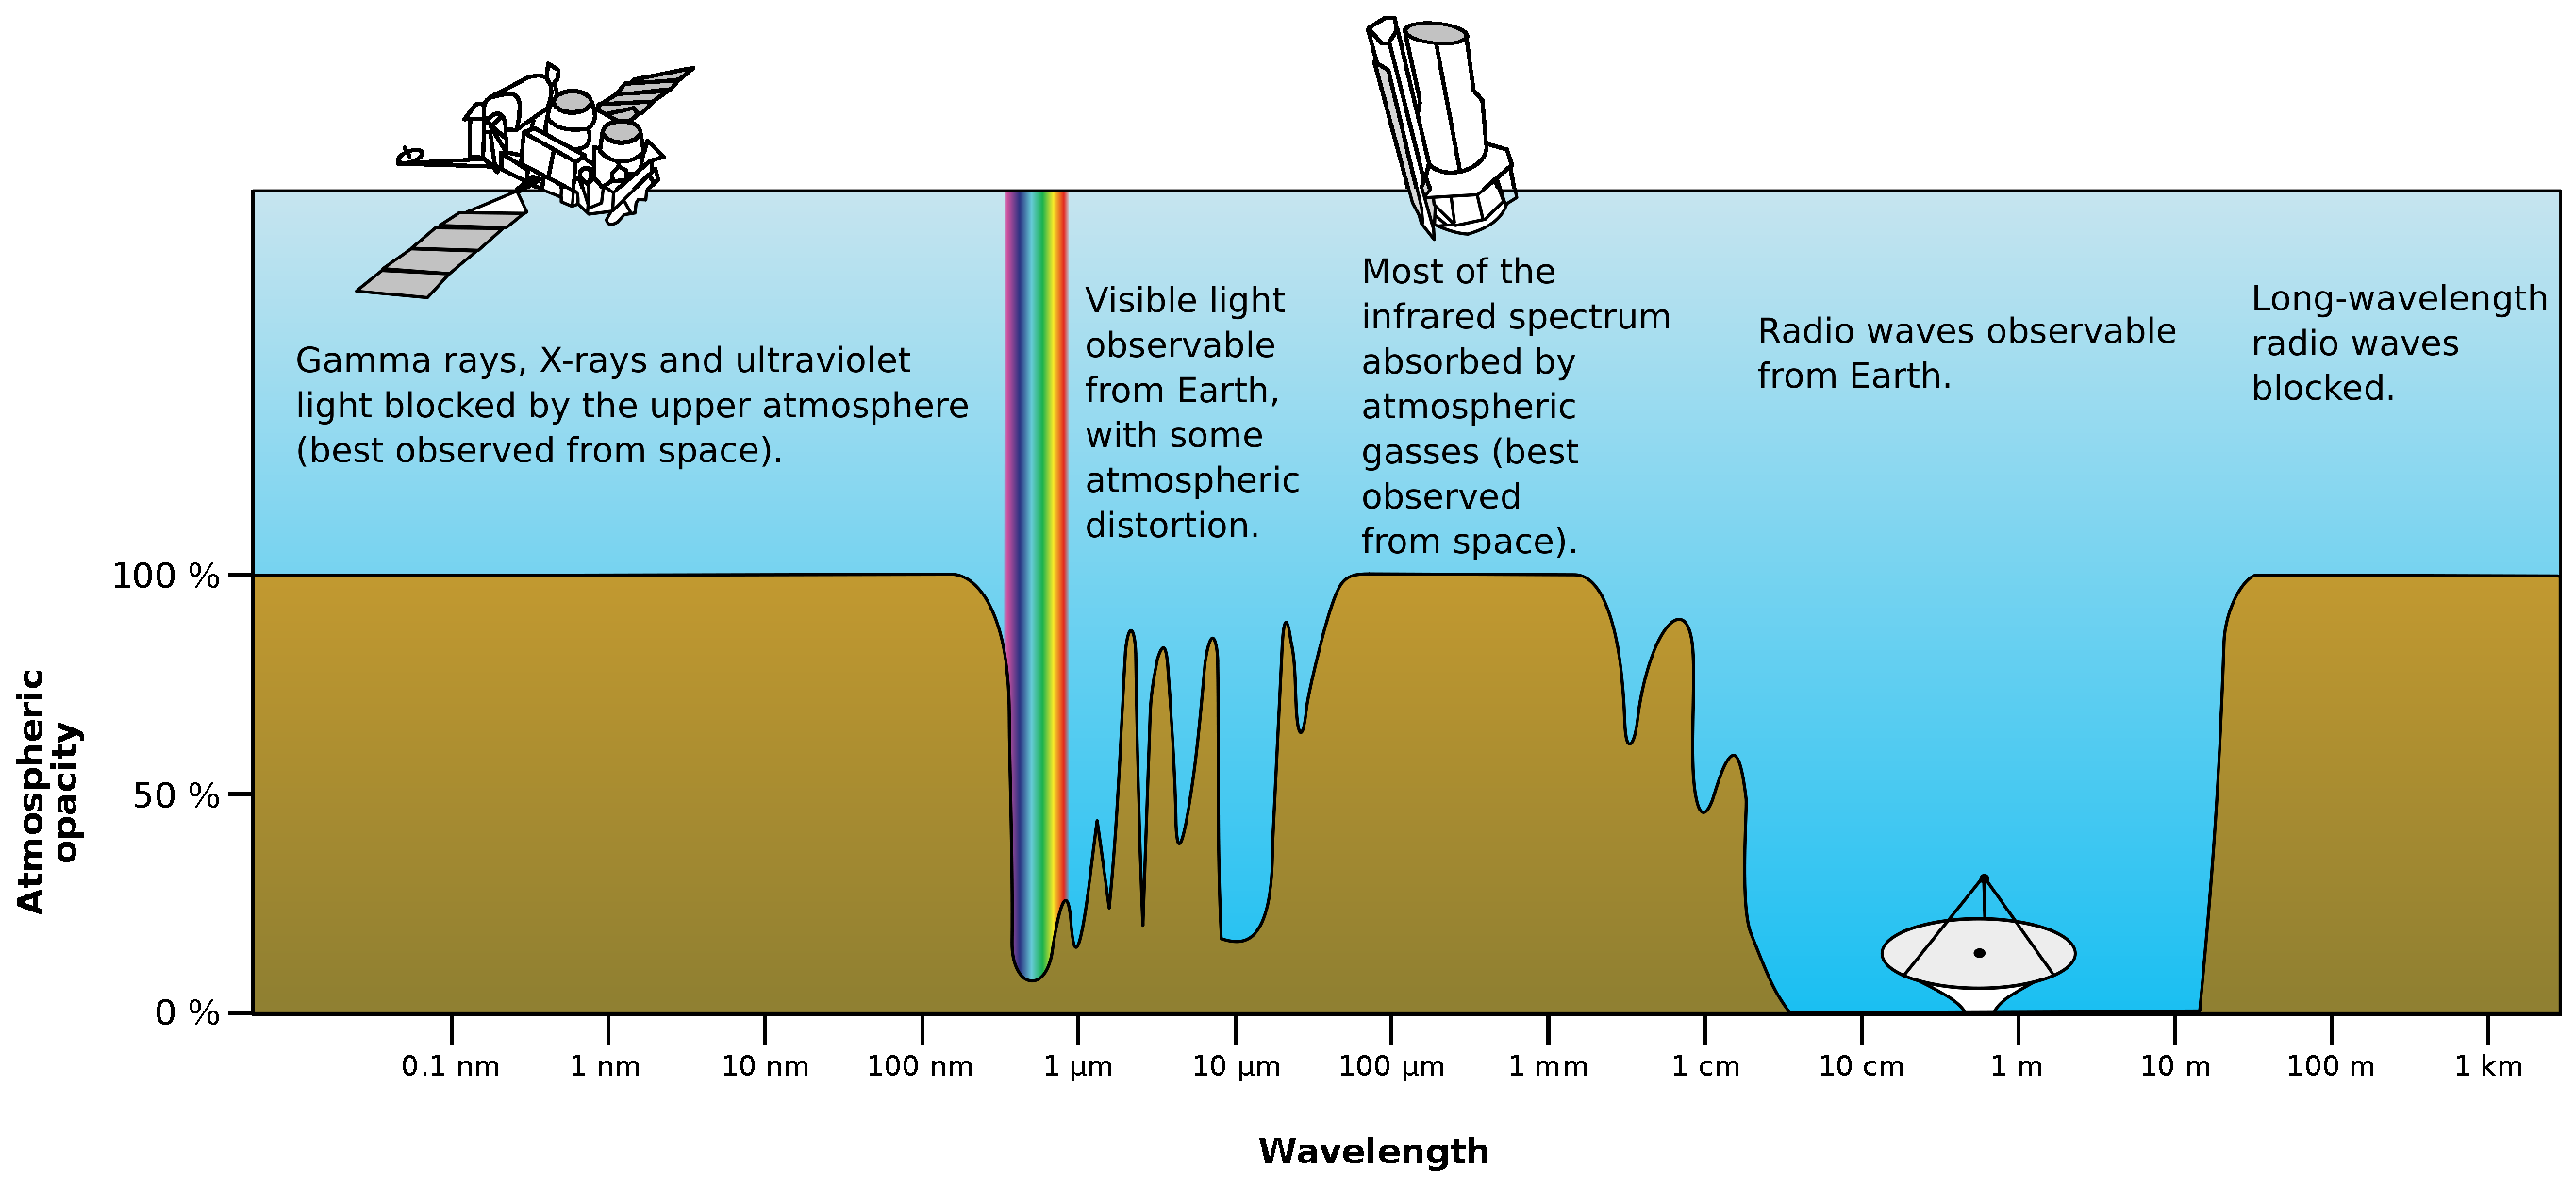
\includegraphics[width=0.7\textwidth]{img/Atmospheric_electromagnetic_opacity}
	\end{center}
	Le altre onde elettromagnetiche vengono in gran parte assorbite dall'atmosfera
	terrestre.
\end{frame}

\begin{frame}{I radiotelescopi di Medicina}
	\only<2>{ \pgfputat{
		\pgfxy(5.5,0)}{
			\pgfbox[left,base]{
				\includegraphics[width=0.45\textwidth]{img/croce_del_nord}
			}
		}
	}
	\only<3>{ \pgfputat{
		\pgfxy(5.5,0) }{
			\pgfbox[left,base]{
				\includegraphics[width=0.45\textwidth]{img/parabolica}}
			}
		}
\end{frame}

\section{Il software}
\subsection{Modularità}
\subsection{Threading}
\section{Risultati e Conclusioni}
\subsection{Risultati dei test}
\subsection{Conclusioni}
\subsection{Sviluppi futuri}
\end{document}
